\documentclass[border=10pt]{standalone}
\usepackage{tikz}\usepackage{amsmath}\usetikzlibrary{arrows.meta}
\begin{document}
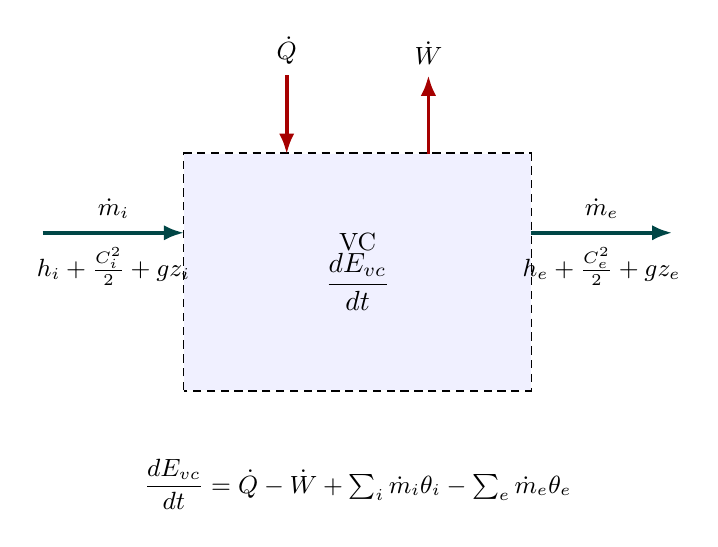
\begin{tikzpicture}[line width=1pt,>={Latex[length=2.6mm]}]
  \draw[densely dashed,line width=1.2pt] (0,0) rectangle (4.4,3.0);
  \fill[blue!6] (0,0) rectangle (4.4,3.0);
  \node[align=center] at (2.2,1.5){\small VC\\$\dfrac{dE_{vc}}{dt}$};
  % entrada (energia de flujo)
  \draw[->,teal!55!black,line width=1.5pt] (-1.8,2.0)--(0,2.0);
  \node[above] at (-0.9,2.05){\small $\dot m_i$}; \node[below] at (-0.9,1.95){\small $h_i+\tfrac{C_i^2}{2}+gz_i$};
  % salida
  \draw[->,teal!55!black,line width=1.5pt] (4.4,2.0)--(6.2,2.0);
  \node[above] at (5.3,2.05){\small $\dot m_e$}; \node[below] at (5.3,1.95){\small $h_e+\tfrac{C_e^2}{2}+gz_e$};
  % Q y W
  \draw[->,red!65!black,line width=1.3pt] (1.3,4.0)--(1.3,3.0); \node[above] at (1.3,4.0){\small $\dot Q$};
  \draw[->,red!65!black,line width=1.3pt] (3.1,3.0)--(3.1,4.0); \node[above] at (3.1,4.0){\small $\dot W$};
  \node[align=center] at (2.2,-1.2){\small $\dfrac{dE_{vc}}{dt}=\dot Q-\dot W+\sum_i\dot m_i\theta_i-\sum_e\dot m_e\theta_e$};
\end{tikzpicture}
\end{document}
